\section{Modellazione generativa e discriminativa a confronto} 



Per una più accurata comprensione della modellazione generativa si rende opportuno un confronto con la controparte: la \emph{modellazione discriminativa}.

In Figura~\ref{fig:discr_model} è riportato un modello discriminativo atto a 
discernere se la paternità di un dipinto è o no attribuibile a Van Gogh. 
\begin{figure}
    \centering
    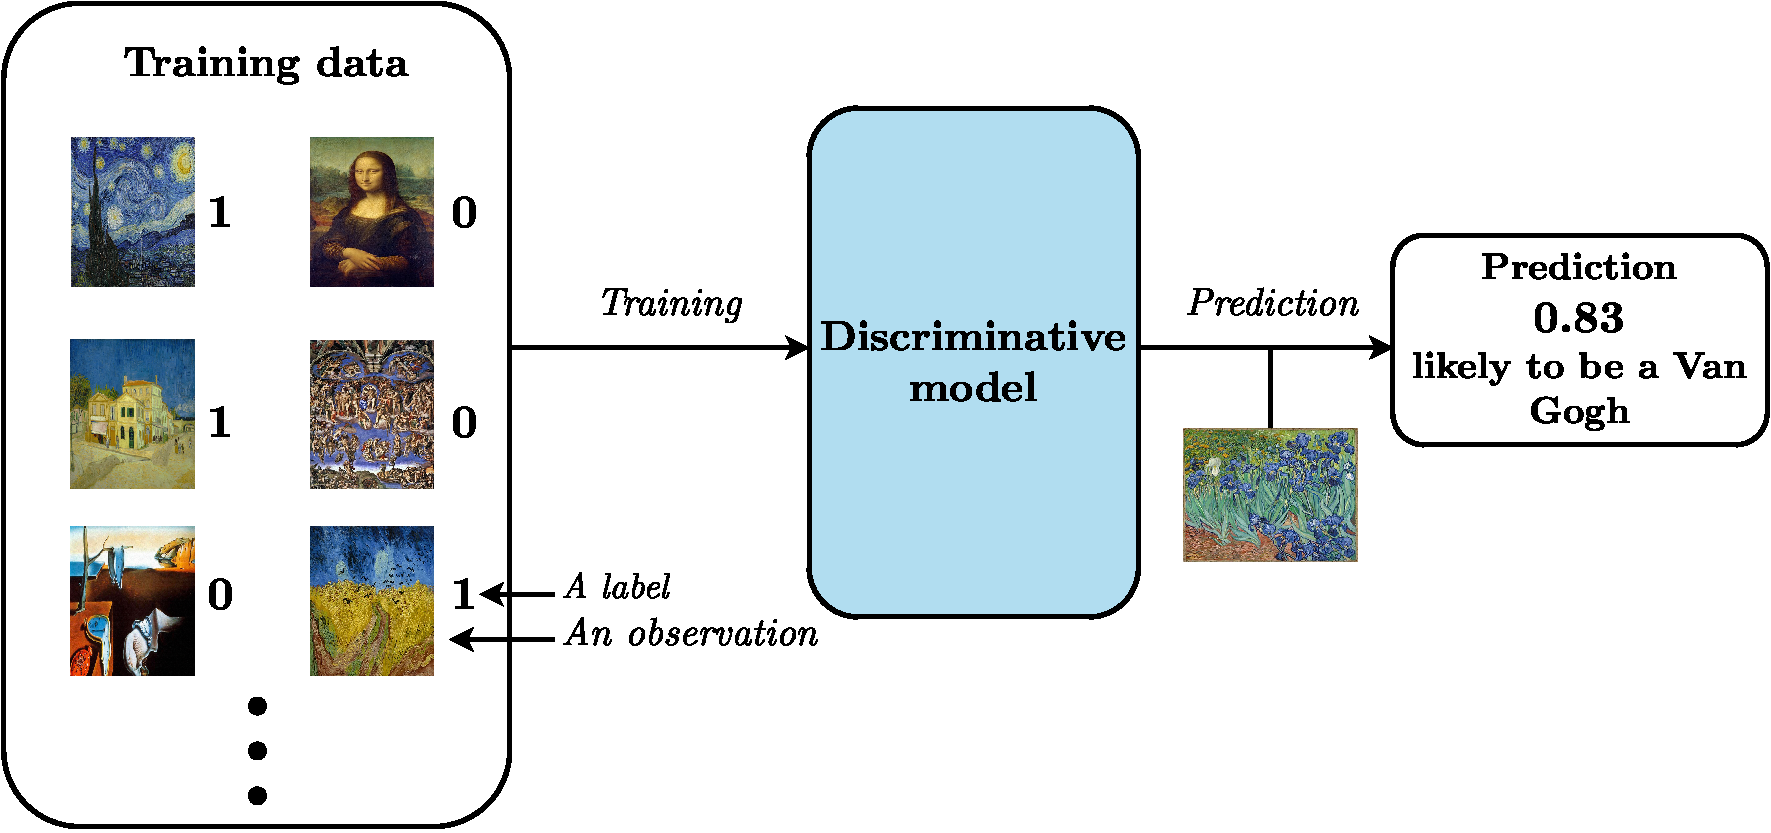
\includegraphics[keepaspectratio, scale=0.45]{Discriminative_model}
    \caption{Modello discriminativo addestrato a predire se una data immagine è stata dipinta da Van Gogh. Fonte:~\cite{fosterGenerativeDeepLearning2023}.}
    \label{fig:discr_model}
\end{figure}
Trattandosi di un tipico problema di classificazione binaria, il dataset di addestramento viene suddiviso in due gruppi:
i dipinti di Van Gogh vengono etichettati con $1$, laddove i dipinti di altri artisti sono etichettati con $0$. 
Il suddetto modello viene quindi addestrato a \emph{discriminare} tra i due gruppi e restituisce la probabilità 
che un'immagine, non presente nel dataset di addestramento, abbia come etichetta $1$(i.e.\ sia effettivamente un quadro di Van Gogh)~\cite{fosterGenerativeDeepLearning2023}.

\noindent Si noti come, nel contesto della modellazione discriminativa, ogni osservazione nel dataset di addestramento sia corredata da un'etichetta (\emph{label}).
Di converso, l'etichettatura del dataset di addestramento non costituisce un requisito essenziale nell'ambito della modellazione generativa, concernente la 
creazione di immagini inedite piuttosto che la corretta attribuzione dell'etichetta ad una data immagine.

\bigskip
\noindent Di seguito si formalizza matematicamente quanto appena esposto:
\begin{itemize}
\item i modelli discriminativi stimano la probabilità $p(y|\mathbf{x})$ che $y$ sia l'etichetta corrispondente ad una data osservazione $\mathbf{x}$ (Figura~\ref{fig:discr_model}).
\item i modelli generativi stimano la distribuzione incognita $p(\mathbf{x})$ dei dati del dataset di addestramento: il modello genera, quindi, nuovi dati a partire dalla distribuzione appresa.
\end{itemize}



\begin{oss}
Si noti che un modello generativo può anche stimare la probabilità condizionata $p(\mathbf{x}|y)$ di osservare il dato $\mathbf{x}$ la cui etichetta è $y$. 
Ad esempio, se il dataset di addestramento contenesse immagini di diversi tipi di alberi, si potrebbe ricorrere ad un modello generativo per generare un'immagine di un cipresso: in tal caso si parla di 
\emph{modelli generativi condizionati}~\cite{fosterGenerativeDeepLearning2023}.
\end{oss}


\noindent Dunque, mentre l'obiettivo della modellazione discriminativa è quello di classificare i dati in base alle loro caratteristiche (\emph{features}), 
la modellazione generativa concerne la creazione di nuovi dati che esibiscono affinità con il dataset di addestramento.

